\documentclass[12pt]{report}

% Paquetes LaTeX y estilos globales
\usepackage[utf8]{inputenc}
\usepackage{multicol}
\usepackage{xcolor}
\usepackage{subfigure}
\usepackage[spanish]{babel}
\usepackage[utf8]{inputenc}
\usepackage{graphicx}
\usepackage{titlesec}
\usepackage[bookmarks,breaklinks,colorlinks=true,allcolors=blue]{hyperref}
\usepackage{listings}
\usepackage{inconsolata}
\usepackage{float}

\usepackage[square,numbers]{natbib}
\AtBeginDocument{
  \renewcommand{\bibsection}{\chapter{\bibname}}
} % Bibliografia en capitulo numerado

\usepackage{geometry}
\usepackage{amsmath}
\usepackage{parskip}
\usepackage[official]{eurosym}
\usepackage{todonotes}
\usepackage{csquotes}

% Formato del título de capítulos y secciones
\titleformat{\chapter}[block]{\titlerule[0.8pt]\normalfont\huge\bfseries}{\thechapter.}{.5em}{\Huge}[{\titlerule[0.8pt]}]
\titlespacing*{\chapter}{0pt}{-19pt}{25pt}
\titleformat{\section}[block]{\normalfont\Large\bfseries}{\thesection.}{.5em}{\Large}



% Formato del código fuente con lstlisting
\lstset{
  basicstyle=\ttfamily,
  breaklines=true,
}

% Márgenes
\geometry{
    a4paper,
    margin=2.95cm
}

% Limite de profundidad del índice
\setcounter{tocdepth}{2}

% Indentación de párrafos
\setlength{\parindent}{1.2cm}

\renewcommand{\lstlistingname}{Extracto de código}
\renewcommand*{\lstlistlistingname}{Índice de extractos de código}

% Comienzo del documento
\begin{document}

    % Portada y secciones no numeradas
    \begin{center}

\vspace*{1cm}


\includegraphics[width=\textwidth]{fig/ETSE.png}

\vspace*{3cm}
\begin{large}
TRABAJO FIN DE MÁSTER
\end{large}

\vspace*{0.1in}
\textbf{\huge Desarrollo de un entorno de trabajo aplicado al desarrollo de firmware para robots móviles} % Aquí el título de su trabajo

\vspace*{.2in}

{\large Realizado por:}\\
\vspace*{0.2cm}\
\textbf{\Large Rubén Garrido Alonso} % Aquí su nombre

\vspace*{2cm}

%\textbf{Para la obtención del título de}\\
{\LARGE Máster Universitario en Ingeniería Electrónica} % Dejar sólo la que corresponda

\vspace*{0.2in}
\textbf{Dirigido por:}\\\
\vspace*{0.2cm}\\
{\large Vicent Girbés Juan}\\ % Repetir esta línea si hay más de un tutor
{\large Valero Laparra Pérez-Muelas}\\

\vspace*{0.2in}

\textbf{Realizado en el departamento de}\\
{\large Ingeniería Electrónica}

\vspace*{.6in}
\textbf{\Large Julio, 2022} % Adaptar al curso en el que presente el trabajo

\end{center}


%\thispagestyle{empty} % Impide que se incluya número de página en la portada
%\clearpage\setcounter{page}{1} % Comienza a incluir números de página a partir de aquí
\pagenumbering{roman} % En números romanos

    \chapter*{Agradecimientos}
Quiero agradecer a X por...

También quiero agradecer a Y por...
    \chapter*{Resumen}
Incluya aquí un resumen de los aspectos generales de su trabajo, en español.

\vspace{.5cm}

\textbf{Palabras clave:} Palabra clave 1, palabra clave 2, ..., palabra clave N
    \chapter*{Abstract}
This section should contain an English version of the Spanish abstract.

\vspace{.5cm}

\textbf{Keywords:} Keyword 1, keyword 2, ..., keyword N
    
    % Índice del documento y de figuras
    \begingroup
        % Los enlaces son normalmente azules, pero en los índices se configuran a negro
        % para que no aparezca todo azul
        \hypersetup{linkcolor=black}
        \tableofcontents
        \listoffigures
        \lstlistoflistings
    \endgroup
    
    % Cambia el estilo de números de página a normal
    \clearpage\pagenumbering{arabic}
    
    % Capítulos del trabajo
    %\chapter{Introducción}\label{cap:ejemplos}

\todo[inline]{Este capítulo se incluye únicamente como ayuda y referencia de uso de \LaTeX. No debe aparecer en el documento final.}

\section{Introducción}
En este capítulo se muestran ejemplos de uso de \LaTeX para operaciones comunes. 

\section{Estilos}\label{sec:estilos}
Se pueden aplicar estilos al texto como \textbf{negritas}, \textit{cursiva} y \underline{subrayado}. También se \textcolor{red}{pueden} \textcolor{blue}{aplicar} \textcolor{green}{colores}, y \underline{\textit{combinar}} \textbf{\textcolor{red}{estilos}}. Se recomienda usar sólo negritas para hacer énfasis, y no abusar de este recurso.

\section{Listados}
Con itemize se pueden crear listas no numeradas:

\begin{itemize}
    \item Fresas
    \item Melocotones
    \item Piñas
    \item Nectarinas
\end{itemize}

De manera similar, enumerate permite crear listas numeradas:

\begin{enumerate}
    \item Elaborar la memoria del TFG
    \item Elaborar la presentación
    \item Presentar el TFG
    \item Solicitar el título de Grado
\end{enumerate}

\section{Subsecciones}
Se pueden definir subsecciones con el comando subsection:

\subsection{Primera subsección}\label{sec:subseccion}
Esto es una subsección

\subsection{Segunda subsección}
Esto es otra subsección.

\section{Imágenes y figuras}
Todas las imágenes y figuras del documento se incluirán en la carpeta ``fig''. Se pueden incluir de la siguiente manera:

\begin{figure}[htp]
    \centering

    \caption{Un feroz depredador}
    \label{fig:ejemplo}
\end{figure}

Observe que las figuras se numeran automáticamente según el capítulo y el número de figuras que hayan aparecido anteriormente en dicho capítulo. Existen muchas maneras de definir el tamaño de una figura, pero se aconseja utilizar la mostrada en este ejemplo: se define el ancho de la figura como un porcentaje del ancho total de la página, y la altura se escala automáticamente. De esta manera, el ancho máximo de una figura sería 1.0 * textwidth, lo que aseguraría que se muestra al máximo tamaño posible sin sobrepasar los márgenes del documento.

Tenga en cuenta que LaTeX intenta incluir las figuras en el mismo sitio donde se declaran, pero en ocasiones no es posible por motivos de espacio. En esos casos, LaTeX colocará la figura lo más cerca posible de su declaración, puede que en una página diferente. Esto es un comportamiento normal y no debe ser evitado.

\section{Referencias}
Observe cómo en el código fuente de esta sección se ha usado varias veces el comando ``label''. Este comando permite marcar un elemento, ya sea capítulo, sección, figura, etc. para hacer una referencia numérica al mismo. Para referenciar una ``label'' se usa el comando ``ref'' incluyendo el nombre de la referencia:

Este es el capítulo \ref{cap:ejemplos}.

En la sección \ref{sec:estilos} se muestran ejemplos de estilos.

La subsección \ref{sec:subseccion} explica...

En la Figura \ref{fig:ejemplo} vemos que...

Esto evita que tengamos que escribir directamente los índices de las secciones y figuras que queremos mencionar, ya que LaTeX lo hace por nosotros y además se encarga de mantenerlos actualizados en caso de que cambien (pruebe a mover este capítulo al final del documento y observe cómo se actualizan automáticamente todos los índices referenciados). Además, las referencias mediante ``ref'' actúan como hipervínculos dentro del documento que llevan al elemento referenciado al pulsar en ellas.

Es habitual nombrar las ``label'' con un prefijo que indica el tipo de elemento para encontrarlo luego más fácilmente, pero no es obligatorio.

\section{Extractos de código}

Se pueden incluir extractos de código mediante lstlisting:

\begin{lstlisting}[language=Python, caption={Código Python}, label={cod:python}, captionpos=b]
num = float(input("Enter a number: "))
if num > 0:
   print("Positive number")
elif num == 0:
   print("Zero")
else:
   print("Negative number")
\end{lstlisting}

Se admite gran variedad de lenguajes:

\begin{lstlisting}[language=Java, caption={Código Java}, label={cod:java}, captionpos=b]
public class Test {
    public static void main(String[] args) {
        System.out.println("Hello, world!");
    }
}
\end{lstlisting}

Los extractos de código también se pueden referenciar mediante label/ref: Extractos de código \ref{cod:python} y \ref{cod:java}.

\section{Enlaces}
Puede enlazar una web externa mediante el comando url: \url{https://www.example.com}. También se puede vincular un enlace a un texto mediante el comando href: \href{https://www.example.com}{dominio de ejemplo}.

\section{Citas y bibliografía}
En LaTeX, los elementos de la bibliografía se almacenan en un fichero bibliográfico en un formato llamado BibTeX, en el caso de este proyecto se encuentran en ``bibliografia.bib''. Para citar un elemento se usa el comando ``cite''. Se pueden citar tanto artículos científicos \cite{borrego2019} como enlaces web \cite{webETSII}. Las citas se numeran automáticamente y se incluyen en la sección de bibliografía del documento.

Observe cómo los elementos bibliográficos almacenados en ``bibliografia.bib'' tienen una etiqueta asociada, que es la que se incluye al citarlos mediante cite. Añadir una referencia al fichero bibliográfico no hace que ésta aparezca automáticamente en la sección de bibliografía del trabajo, es necesario citarla en algún lugar del mismo.

\section{Ecuaciones}
LaTeX tiene un potente motor para mostrar ecuaciones matemáticas y un amplio catálogo de símbolos matemáticos. El entorno matemático se puede activar de muchas maneras. Para incluir ecuaciones simples en un texto se pueden rodear de símbolos dólar: $1 + 2 = 3$, $\sqrt{81} = 3^2 = 9$, $\forall x \in y~\exists~z : S_z < 4$.

Las ecuaciones más complejas pueden expresarse aparte y son numeradas: ecuación \ref{eq:ecuacion}.

\begin{equation}\label{eq:ecuacion}
\lim_{x\to 0}{\frac{e^x-1}{2x}}
 \overset{\left[\frac{0}{0}\right]}{\underset{\mathrm{H}}{=}}
 \lim_{x\to 0}{\frac{e^x}{2}}={\frac{1}{2}}
 +7 \int_0^2
  \left(
    -\frac{1}{4}\left(e^{-4t_1}+e^{4t_1-8}\right)
  \right)\,dt_1
\end{equation}

Dispone \href{http://www.yann-ollivier.org/latex/texsymbols.pdf}{aquí} de un amplio listado de símbolos que pueden usarse en modo matemático.

\section{Caracteres y símbolos especiales}
Algunos caracteres y símbolos deben ser escapados para poder representarse en el documento, ya que tienen un significado especial en LaTeX. Algunos de ellos son:

\begin{itemize}
    \item El símbolo dólar \$ se usa para ecuaciones.
    \item El tanto por ciento \% se usa para comentarios en el código fuente.
    \item El símbolo euro \euro{} suele dar problemas si se escribe directamente.
    \item El guión bajo \_ se usa para subíndices en modo matemático.
    \item Las comillas deben expresarse `así' para comillas simples y ``así'' para comillas dobles. Las comillas españolas pueden expresarse \textquote{así}.
    \item La barra invertida o contrabarra \textbackslash{} se usa para comandos LaTeX.
    \item Otros símbolos que deben escaparse son las llaves \{ \}, el ampersand \&, la almohadilla \# y los símbolos mayor que \textgreater{} y menor que \textless{}.
\end{itemize}
    \chapter{Introducción}\label{cap:introduccion}
\section{Introducción} 
Cada vez es mayor el peso que la tecnología esta teniendo en el día a día de la sociedad. La interacción con dispositivos tecnológicos está convirtiéndose poco a poco en algo cotidiano. Son cada vez mas las tareas que pueden ser suplidas por dispositivos electrónicos que ayudan a que tareas del día a día, incluso labores más peligrosas puedan desarrollarse de una forma segura y eficiente.

Uno de los sectores en auge en esta última década es el sector de los sistemas embebidos y la capacidad de procesamiento de estos mismos, es cada vez mayor la capacidad de dotar de inteligencia a dispositivos cada vez con dimensiones mas reducidas pero con una capacidad de rendimiento que crece de forma exponencial.

El proyecto que se describirá a lo largo de la memoria se encarga de dotar de inteligencia artificial un robot con capacidad de teleoperación y reconocimiento del entorno en el cual se esté operando este mismo. Para poder conseguir esto, se ha tenido que poner a punto un robot que sea capaz de moverse y además sea capaz de procesar y reconocer los objetos de su entorno procesando esta información en tiempo real.

Para conseguir esto se ha dotado al robot de visión artificial, la cual recogerá la información necesaria de una cámara incorporada en el robot y que se complementará con otros sensores que ayudaran al dispositivo móvil a poder moverse de una forma autónoma evitando colisiones.


\section{Motivación del proyecto} 
La motivación del proyecto surge con el auge del desarrollo de robots móviles junto con el actual desarrollo de dispositivos dotados de inteligencia artificial o ''capacidad de aprendizaje'' en estas máquinas. 

Con el objetivo de hacer mas accesible el proyecto a toda la comunidad se ha tratado de utilizar hardware abierto, así como intentar utilizar plataformas de software open source.

tras recopilar información sobre el funcionamiento de diferentes tipos de robots móviles, vehículos auto-guiados y diversos dispositivos de conducción autónoma, se ha tratado de comprender y estudiar su funcionamiento interno, desde el desarrollo de hardware de cada uno de los robots hasta comprender la estructura de software que cada un de los diferentes dispositivos puede contener. De este modo, una vez estudiadas las diferentes alternativas que se encuentran actualmente accesibles en el mercado, se ha tratado de proporcionar una solución accesible, que cuente con cierta escalabilidad y que sirva como plataforma de desarrollo para demás desarrolladores. 

Para poder desarrollar ciertas soluciones para diferentes tipos de robots, siempre se han de tener en cuenta las diferentes versiones de todas y cada una de las dependencias que el programa a desarrollar puede tener. También es cierto, que hoy en día existen diversas tecnologías que permiten encapsular todas aquellas dependencias en un entorno estable para que todos los desarrolladores de un mismo proyecto cuenten con las mismas herramientas y programas, actualizadas a la misma versión, de esta forma se eliminan problemas de retrocompatibilidad entre diferentes desarrolladores y los prototipos a desarrollar.

\section{Objetivo del proyecto} 

El objetivo del proyecto es dotar a los usuarios desarrolladores de un entorno encapsulado con todas las herramientas necesarias para poder llevar a cabo el desarrollo programas y nuevas funcionalidades en el marco del desarrollo de robots móviles.

Para ello, la plataforma de desarrollo debe de ser estable y permitir un esquema multiusuario, donde cada uno de los desarrolladores pueda llevar a cabo sus labores con total comodidad y sin conflictos con las versiones desarrolladas por otros usuarios.

Dado que el objetivo principal es implantar un entorno estable y para usar por diferentes usuarios, debe de ser de fácil acceso y fácil instalación para todos los usuarios.
 \section{Marco teórico}
 
El robot utilizado para el proyecto alberga diferentes bloques de funcionamiento o diferentes secciones que trabajaban de forma paralela para poder conformar el proyecto. Es por ello que se debe tener claro desde el inicio del proyecto la forma en la que se va a establecer la comunicación entre los diferentes nodos del proyecto o las diferentes partes que albergan diferente hardware.

Dado el el dispositivo que se quiere desarrollar es un robot, se ha optado por utilizar un sistema operativo de software abierto llamado ROS (Robot Operative System).

Dicho sistema operativo se ejecuta sobre una CPU bajo un sistema Linux basado en una distribución Debian. 

El proyecto a desarrollar se divide en dos grandes bloques:

\begin{itemize}
\item Alto nivel : Lo forman los dispositivos que albergarán las lógicas de navegación así como la parte mas abstraída del Hardware. Prácticamente toda la inteligencia del robot estará contenida en este bloque. Para poder desarrollar el alto nivel se han utilizado dos Raspberrys, las cuales ejecutarán la lógica de funcionamiento del robot así como el "cerebro" del robot ejecutando el framework ROS. 

El el alto nivel también se encuentran diferentes sensores cuya información necesita ser procesada por una CPU y que son utilizados para poder ejercer una navegación más fina así como poder almacenar un mapa de los diferentes entornos por los que ha estado navegando.


\item Bajo nivel : El bajo nivel contiene la lógica necesaria para poder realizar la gestión entre los sensores y actuadores y la lógica que cada uno de estos necesita para su correcto funcionamiento. El bajo nivel esta ligado al hardware y alberga la parte de programación que gestiona de una forma mas directa la mayoría de sensores y de actuadores. 
\end{itemize}

El bajo nivel lo conforma entre otros, el microcontrolador de Arduino utilizado para el proyecto.

Para poder realizar la detección de objetos y personas, se empleará un modelo de inteligencia artificial. Se realizará una comparativa entre los diferentes tipos de modelos y tipologías a la hora de realizar una detección de objetos.

El procesado de toda la información que se lleve a cabo para poder procesar la imagen adquirida por la cámara así como la información que servirá como input al modelo de inteligencia artificial, se procesará en el mismo robot. A esta técnica se le conoce como "edge computing".
    \chapter{Entorno Software}\label{cap:planificación}
Tal y como se menciona a lo largo de la memoria, el desarrollador debe de tener una estructura y un entorno de trabajo que garantice la correcta funcionalidad de todas las herramientas facilitadas para el desarrollo. 

Son diferentes las herramientas que se prepararán a lo largo de la memoria, todas las herramientas, funcionan bajo licencias de software libre, y son completamente gratuitas de utilizar. Dado que el entorno está orientado a el desarrollo de firmware para robot móviles, el entorno se encapsulará para que todo se ejecute sobre el sistema operativo Linux. El motivo por el que se ha elegido Linux como base de desarrollo es por ser el sistema operativo principal para el desarrollo de software, ya que está construido bajo licencias de software libre.

Para el desarrollo de 
\section{Linux}
\section{ROS}
\section{Entorno desarrollo Robot}

\subsection{Puesta a punto Coral TPU}

Con el objetivo de poder llevar a cabo la detección de objetos a tiempo real, se ha hecho uso de un acelerador gráfico USB, en concreto un dispositivo TPU (Tensor Procesor Unit) el cual se encargará de poder llevar a cabo el cálculo y procesado relacionado con la detección de objetos y la aplicación y procesado del modelo matemático.

Para poder llevar a cabo el procesamiento de las imágenes y el cálculo estructural de la red neuronal, se utilizan dispositivos a los que comúnmente se les denomina acelerador gráfico. Estos dispositivos se encargar de soportar el peso computacional correspondiente a los cálculos asociados a los modelos matemáticos. En este caso, el gran parte del peso del procesado recae sobre el modelo matemático y su procesado en CPU, es por ello, que para obtener unos mejores tiempos de respuesta y poder llevar a cabo un procesado en tiempo real y con una latencia baja se utilice una TPU.

\begin{figure}[h]
    \centering
    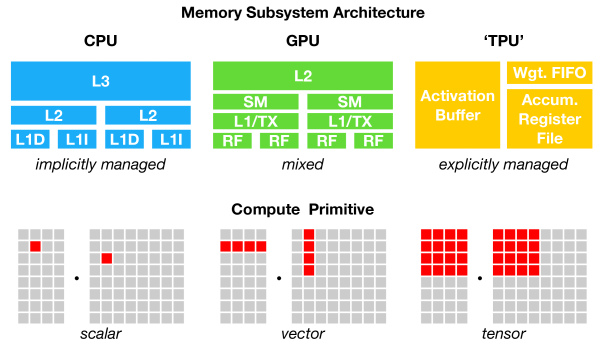
\includegraphics[scale=0.5]{fig/tpuVScpu.png}
    \caption{Comparativa CPU, GPU y TPU.}
    \label{fig:mesh1}
\end{figure}

Tal y como se puede observar en la figura XX, cada una de los diferentes tipos de procesadores destaca en un ámbito diferente y cada un o tiene su aplicaciones particular. En lo que atañe al proyecto, ya que la carga de trabajo con mayor peso recae sobre el modelo de inteligencia artificial, la mejor opción para poder ejecutar todos estos cálculos de la manera más eficiente es utilizar una TPU.

Las TPU son capaces de procesar la información de modelos matemáticos, como por ejemplo las redes neuronales, de 15 a 30 veces mas rápido que una GPU convencional, además de ser mas eficientes energéticamente debido a su bajo consumo. El inconveniente de estos dispositivos es la baja versatilidad a la hora de incluirlos en el proyecto. Para la aplicación deseada encaja perfectamente debido al tipo de procesado que realizará, el bajo coste económico y la fácil instalación del dispositivo en el sistema operativo gracias a su conexión USB 3.0. 

\begin{figure}[h]
    \centering
    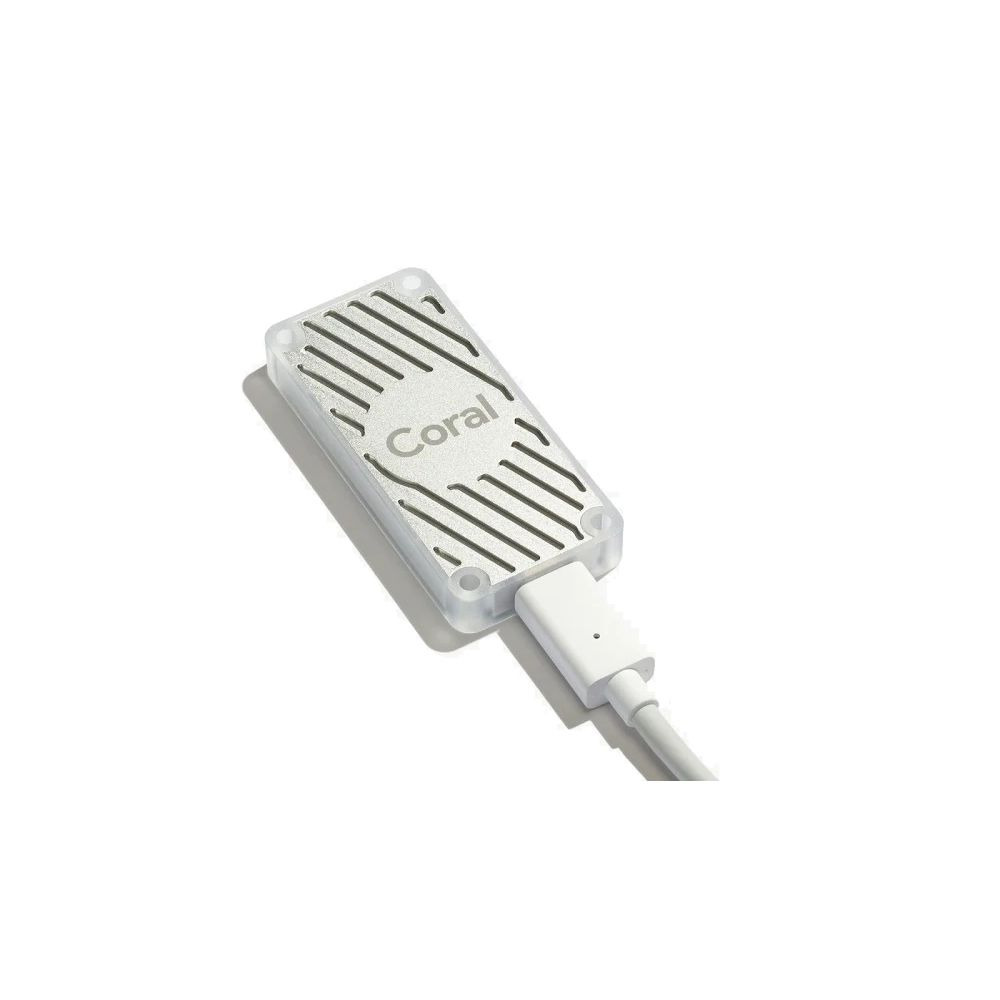
\includegraphics[scale=0.5]{fig/google_coral_usb_accelerator_1.jpg}
    \caption{Google Coral TPU USB Accelerator.}
    \label{fig:mesh1}
\end{figure}

Para poder poner en funcionamiento la TPU se deben de cumplir una serie de requisitos software para que el sistema operativo sea capaz de trabajar con el hardware. Es necesario instalar una serie de drivers para que se pueda establecer un entendimiento hardware-software y de esa forma poder realizar la mayor parte del procesado en este hardware.

Para poner a punto la Coral TPU y poder comprobar su correcto funcionamiento, el primero de los pasaos a seguir es instalar un gestor de paquetes para poder resolver todas las dependencias que se vayan necesitando a lo largo de la instalación y puesta a punto. En el caso de los proyectos, se ha instalado conda para poder gestionar entornos e instalar los diferentes paquetes para python que se van necesitando a lo largo de la puesta en marcha. 

\begin{figure}[h]
    \centering
    
\includegraphics[scale=0.5]{fig/python-conda.png}
    \caption{Gestor de paquetes y entornos Conda.}
    \label{fig:mesh1}
\end{figure}

Se ha de tener en cuenta la distribución y arquitectura que presentará el proyecto a la hora de poder instalar un paquete determinado ya que dependiendo de cada arquitectura, distribución y kernel de cada uno de los sistemoas operativos y harware que se esté utilizando se deberá de adaptar a un software y otro.

Para el caso del proyecto, se esta ejecutando todo el código sobre un linux, con una distribución basada en ubuntu server al que se le ha instalado un entorno gráfico. A la hora de instalar el gestor de paquetes Conda hay que tener en cuenta diversos factores diferenciales.

Primero debemos de conocer la arquitectura y la version del sistema operativo sobre el cual estamos ejecutando, para ello se pude abrir una ventana de comandos o terminal y ejecutar el siguiente comando: "uname -m".

\begin{figure}[h]
    \centering
    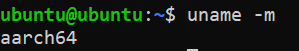
\includegraphics[scale=1.5]{fig/uname -r.PNG}
    \caption{Ejecución de comando "uname -r".}
    \label{fig:mesh1}
\end{figure}

Tal y como se puede observar en la figura XX, el comando uname -r nos muestra en la terminal el tipo de arquitectra sobre el que estamos trabajando. Como era de esperar, Raspberry trabaja con una CPU ARM, por lo cual el resultado de ejecutar el comando es "aarch64".

Para poder instalar conda sobre procesadores ARM habrá que recurir a una versión de conda adaptada para estas arquitecturas, ya que los gestores mas utilizados para poder trabajar con conda, bien sea "Anaconda" o bien "Miniconda" únicamente están disponibles para poder instalarlos sobre procesadores AMD, por lo cual hay que buscar una alternativa o solución a este pequeño inconveniente.

Tras invesigar las diferentes opciones que sencuentran como software abierto por la red, se ha escogido "Archiconda" como gestor de entornos y paquetes de conda. Archiconda es un sofware libre y abierto para poder instalar en dispositivos con arquitectura ARM como suelen ser la mayoría de placas de desarrollo para sistemas embebidos.

Para poder instalar archiconda es necesario descargar un repositorio para posteriormente ejecutar los diferentes comandos necesarios. Con el objetivo de simplificar toda la instalación se ha cogido de un repositorio un bash script para linux que se puede o bien descargar o bien generar desde la propia consola.

Ya que el objetivo es poder dejar toda la información ncesaria en un mismo repositorio, se ha decidido generar un fichero bash script propio para poder almacenarlo en un repositoriop propio.

Para poder crear el fichero se debe de realizar el siguiente procedimiento:

En primer lugar se debe de generar un archivo en linuz con extension .sh, a este fichero se le dará el nombre que el usuario desee, en este caso "installArchiconda.sh".

Una vez creado este fichero, se rellenará con el código o acciones que se deseen ejecutar, en este caso el extracto de código que se desea introducir se puede muestra a continuación.

Una vez el archivo queda generado, se guarda para su posterior ejecución. Para poder dar permiso de ejecución en un sistema linux se utilizará el comando " sudo chmod +x installArchiconda.sh ". De este modo estamos añadimos permiso de ejecución para el fichero y se podrá ejecutar desde la terminal utlizando " ./installArchiconda.sh ". En las siguientes figuras se puede observar el proceso de creación del fichero así como su ejecución.

\begin{lstlisting}[language=bash, caption={Código bash}, label={cod:bash}, captionpos=b]
#! /bin/bash

cd ${HOME}
wget https://github.com/Archiconda/build-tools/releases/download/0.2.3/Archiconda3-0.2.3-Linux-aarch64.sh
sudo sh Archiconda3-0.2.3-Linux-aarch64.sh
rm -rf Archiconda3-0.2.3-Linux-aarch64.sh
cd ~
sudo chown -R $USER archiconda3/
export "PATH=/bin:/usr/bin:$PATH" >> ~/.bashrc 
source ~/.bashrc
conda config --add channels conda-forge
conda -V

\end{lstlisting}

\begin{figure}[h]
    \centering
    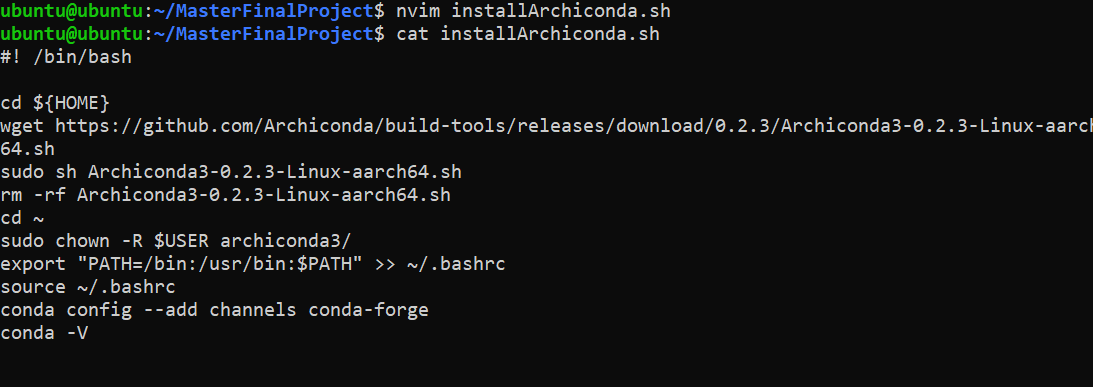
\includegraphics[scale=0.7]{fig/installArchiconda.PNG}
    \caption{Creación archivo instalador archiconda.}
    \label{fig:mesh1}
\end{figure}

\begin{figure}[h]
    \centering
    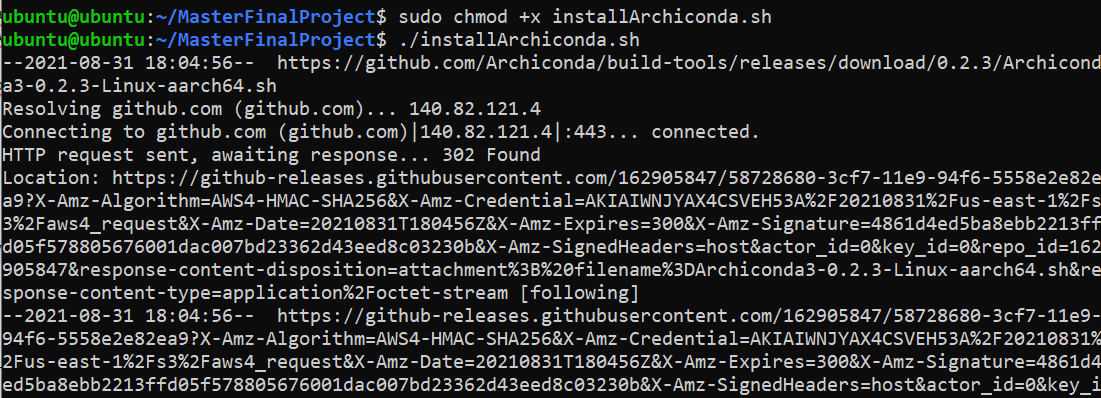
\includegraphics[scale=0.7]{fig/archicondaInstalling.PNG}
    \caption{Ejecución archivo instalador archiconda.}
    \label{fig:mesh1}
\end{figure}

Una vez se ha instalado archiconda, se puede comprobar que se ha instaladao corerrectamente ejecutando el comando " conda --version " o bien " conda -V ". Si este comando devuelve la versión de conda significará que se ha isntalado correctamente y estará todo listo para crear un entorno e instalar los diferentes paquetes necesarios.

Con el gestor de paquetes conda se puede proceder a la instalación y preparación de todo el entorno de desarrollo. El primer de los pasos a seguir para poder poner a punto el proyecto, es crear un entorno aislado donde poder compilar y donde poder alojar todos los paquetes necesarios para que a la hora de ejecutar se puedan encontrar todas las librerías en el entorno adecuado. Para poder hacer esto el primero de los comando a ejecutar es " conda create --name tflite1-env ".
 
 \begin{figure}[h]
    \centering
    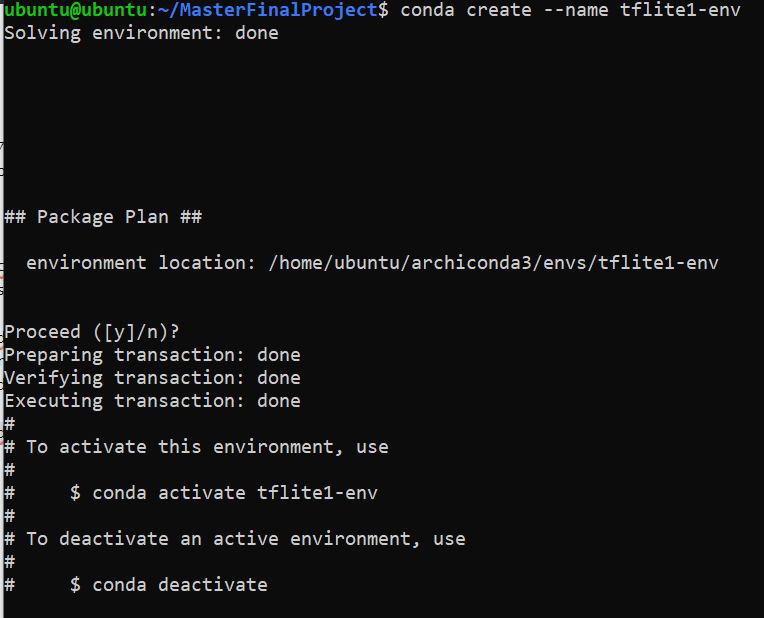
\includegraphics[scale=0.7]{fig/conda create.PNG}
    \caption{Ejecución archivo instalador archiconda.}
    \label{fig:mesh1}
\end{figure}

Una vez creado el entorno conda donde poder ejecutar los comandos, el siguiente paso será poder ejecutar " conda activate tflite1-env ". De esta forma se activa el entorno conda donde se quiere trabajar y estará todo preparado para poder empezar a instalar dependencias.

\begin{figure}[h]
    \centering
    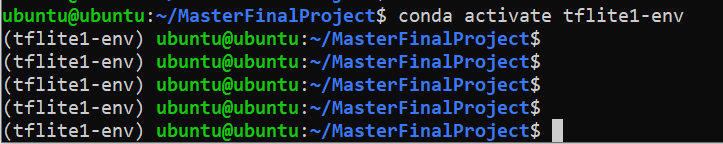
\includegraphics[scale=0.7]{fig/conda activate.PNG}
    \caption{Ejecución archivo instalador archiconda.}
    \label{fig:mesh1}
\end{figure}

El siguiente paso es instalar las dependencias, para poder instalar las dependencias desde un mismo scripts se han seguido los mismos pasos que se han seguido para la instalación de archiconda. Los requerimientos para poder ejecutar la detección de objetos vienen en el siguiente archivo ejecutable:

\begin{lstlisting}[language=bash, caption={Código bash}, label={cod:bash}, captionpos=b]
#!/bin/bash

# Get packages required for OpenCV

sudo apt-get -y install libjpeg-dev libtiff5-dev libjasper-dev libpng12-dev
sudo apt-get -y install libavcodec-dev libavformat-dev libswscale-dev libv4l-dev
sudo apt-get -y install libxvidcore-dev libx264-dev
sudo apt-get -y install qt4-dev-tools libatlas-base-dev

# Need to get an older version of OpenCV because version 4 has errors
pip3 install opencv-python
# pip install opencv-python (If pip3 drops you an error)

# Get packages required for TensorFlow
# Using the tflite_runtime packages available at https://www.tensorflow.org/lite/guide/python
# Will change to just 'pip3 install tensorflow' once newer versions of TF are added to piwheels

#pip3 install tensorflow
# Modded for installin tflite on a RPI4 running ubuntu mate 20.04
version=$(python -c 'import sys; print(".".join(map(str, sys.version_info[:2])))')

if [ $version == "3.7" ]; then
pip3 install --extra-index-url https://google-coral.github.io/py-repo/ tflite_runtime
fi

if [ $version == "3.5" ]; then
pip3 install --extra-index-url https://google-coral.github.io/py-repo/ tflite_runtime
fi
\end{lstlisting}

Una vez instalado el fichero de requierements, la raspberry estará lista para poder ejecutar una red neuronal precompilada. El siguiente de los pasos consiste en poder establecer la Coral TPU como dispositivo que será encargado de poder procesar toda esta información y poder realizar la detección de objetos.

En este punto la Raspberry es capaz de compilar y poder ejecutar la detección de objetos. Esto se puede conseguir tanto desde una entrada de vídeo como puede ser por ejemplo una webcam, o bien se puede conseguir procesar una imagen o vídeo y aplicar los coeficientes de la red neurona para poder clasificar los diferentes inputs que puedan llegar a través del vídeo. 


\subsection{Comunicación entre dispositivos}

Con el objetivo de poder establecer la comunicación entre todos los dispositivos que formarán parte del robot final, se ha decidido establecer una comunicación serie a través de una UART. 


\subsection{Scripts de python}

\subsection{Imagen Linux}
    \section{Entorno de desarrollo software PC}\label{cap:analisis}

En este capítulo se expone la configuración del entorno de programación en Linux, como se estructura el proyecto y las herramientas que el entorno de Linux/Debian ofrece.

La puesta a punto del robot a nivel de software se ha desarrollado en un entorno GNU-Linux utilizando distribuciones Debian-Ubuntu para poder instalar todas las herramientas necesarias para poder desarrollar el software que se va a implantar en el robot. 

\subsection{Sistema operativo Ubuntu}
Con el objetivo de tener todas las herramientas posibles a la hora de desarrollar el proyecto y poder utilizar todas las funcionalidades que un sistema operativo puede ofrecer, se ha desarrollado el proyecto prácticamente en su totalidad utilizando Linux como base del sistema operativo y base de desarrollo tanto en PC como en la CPU que utilizará el robot.

\begin{figure}[h]
    \centering
    
\includegraphics[scale=0.15]{fig/ubuntu.png}
    \caption{Logotipo distribución Ubuntu.}
    \label{fig:mesh1}
\end{figure}

Ubuntu es una de las distribuciones mas famosas del 
\subsection{ROS}
ROS es un framework de código abierto que proporciona una serie de librerías para la gestión de desarrollo software aplicado a robots.

Entre las librerías que ROS ofrece se encuentran librerías orientadas a la abstracción de hardware, gestión de dispositivos de bajo nivel, comunicación entre sistemas... Todas estas funcionalidades que este framework proporciona hacen que la gestión de la arquitectura software del robot sea mucho mas intuitiva y manejable y por lo tanto hacer el proyecto mas escalable y abierto a nuevas funcionalidades.

Otra de la principal ventaja que hace que ROS sea uno de los frameworks mas utilizados para el desarrollo de aplicaciones con robots es la alta capacidad de reutilizar código que ofrece, esto se debe a las diferentes capas de abstracción que se utiliza en el desarrollo que hacen el desarrollo de "nodos" y "paquetes" de ROS sean muy poco o nada dependientes del hardware a utilizar.

\begin{figure}[h]
    \centering
    
\includegraphics[scale=0.2]{fig/ros.jpg}
    \caption{logo ROS framework.}
    \label{fig:mesh1}
\end{figure}

ROS está diseñado para ser lo más ligero posible, esto hace que sea m;as sencillo poder ejecutar este framework con recursos limitados, en este proyecto, ROS estará corriendo sobre una Raspberry Pi, por tanto es otra de las cualidades a tener en cuenta a la hora de escoger herramientas de software aplicadas a este robot.

Hay dos lenguajes soportados para desarrollar paquetes de ROS, se puede desarrollar tanto en C++ como en Python. Esto lo hace aún mas versátil si cabe y más accesible a mas desarrolladores abriendo el campo del desarrollo colaborativo y la reutilización de código.
\subsection{Instalación de paquetes y herramientas necesarias en PC.}
El primer paso para utilizar todas las herramientas de desarrollo necesarias es poner a punto el software que se va a utilizar. Durante todo el proyecto se han desempeñado tareas de programación y elaboración de código, para poder gestionar y llevar un seguimiento del control de versiones del código del proyecto se ha creado un repositorio donde se ha ido subiendo cada un de los diferentes cambios que se van realizando con el paso del tiempo.

La herramienta escogida para realizar el control de versiones ha sido GIT. Una de las ventajas significativas de poder utilizar un software de control de versiones como puede ser GIT, es la portabilidad que le ofrece al código. Al utilizar repositorios como contenedor de todo el código del proyecto, este se puede clonar y ejecutar desde diferentes dispositivo sin ningún problema.

Por tanto, ha resultado ser especialmente útil para poder portar el código entre sistemas operativos así como para poder transportarlo del PC a la Raspberry Pi. De esa forma, todo el proyecto queda contenido en un mismo repositorio, a disposición de todos los usuarios que quieran desarrollar sobre él.

\begin{figure}[h]
    \centering
    
\includegraphics[scale=0.2]{fig/git.png}
    \caption{Logo control de versiones GIT.}
    \label{fig:mesh1}
\end{figure}

Para trabajar con el control de ver siones se debe de seguir una determinada metodología con el objetivo de llevar una desarrollo del proyecto de forma correcta. Generalmente a la hora de desarrollar un proyecto en GIT, se suele hacer de forma colaborativa, donde todo un equipo de desarrollo se verá involucrado en un determinado código. En este caso, solo uno o dos usuarios serán aquellos que hagan modificaciones en el código.

La metodología mas adecuada que se ha escogido para llevar a cabo el proyecto ha sido "Git Flow".
Git Flow es una metodología de trabajo donde el repositorio que aloja el proyecto se estructura en diversas ramas o espacios donde se diferencian diversas partes del código y donde se estructura el código de forma que según la versión o funcionalidad se puede escoger de una forma sencilla. Generalmente la estructura de las diferentes ramas utilizadas es la que se muestra en la FIGURAX.
\begin{figure}[h]
    \centering
    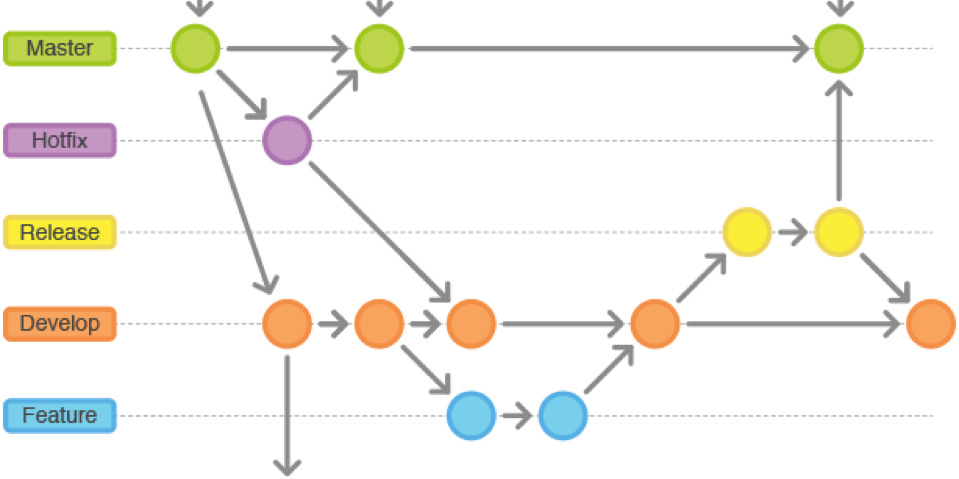
\includegraphics[scale=0.25]{fig/gitFlow.png}
    \caption{Metodología de trabajo ¨Git Flow¨.}
    \label{fig:mesh1}
\end{figure}

Cada una de las ramas alberga el código con las siguientes funcionalidades:
\begin{itemize}
\item Master : Alberga el código que esta actualmente en producción, en este caso alberga el código que se ha utlizado en su versión completamente funcional mas reciente. 
\item Release : Es el último código funcional que se ha enviado para evaluar su calidad y poder enviarlo a producción, también contiene una versión definitiva del código o proyecto a utilizar pero no necesariamente debe de ser el código utilizado en producción.
\item Develop  : Alberga el código que está en actual desarrollo, no necesariamente debe de funcionar a la perfección, aunque es recomendable que todo el código que se pueda descargar de la rama de develop al menos debe de compilar y albergar funcionalidades básicas desarrolladas, aunque en estas se puedan encontrar diferentes bugs. Es la rama donde se encuentra el código antes de mandarlo a la rama de release.
\item Feature : En la rama de feature se desarrollan las nuevas funcionalidades que se van añadir al código.
\end{itemize}


En el caso de este proyecto se ha desglosado en tres ramas, ya que el proyecto no se ha llevado a producción masiva, ha sido suficinete con tener tres ramas diferentes para estructurar de forma correcta el proyecto. En este caso se ha utilizado las ramas "develop" donde se ha ido guardando el código funcional en desarrollo, la rama "feature/" donde se iba desarrollando cada una de las funcionalidades antes de combinarlas con la rama "develop" y por último la rama master, donde se ha ido metiendo el código que era completamente funcional y definitivo.

Otro ámbito importante a la hora de desarrollar el proyecto es poder realizar una correcta depuración de cada una de las partes del proyecto y de cada uno de las diferentes funcionalidades que se van desarrollando a lo largo del proyecto en diferentes ámbitos. Para poder cumplir con este objetivo se han instalado diferentes herramientas que han permitido poder obtener información interesante que verifique el correcto funcionamiento del robot.

En este caso, gran parte de la comunicación establecida entre las diferentes partes del robot, como por ejemplo la comunicación entre el microcontrolador y la Raspberry Pi se han realizado a través de un protocolo UART. La comunicación UART se establece a través de un protocolo serie que se encarga de establecer una comunicación asíncrona donde se envían y reciben datos de forma secuencial a una velocidad determinada, comúnmente llamada "baurate".

\begin{figure}[h]
    \centering
    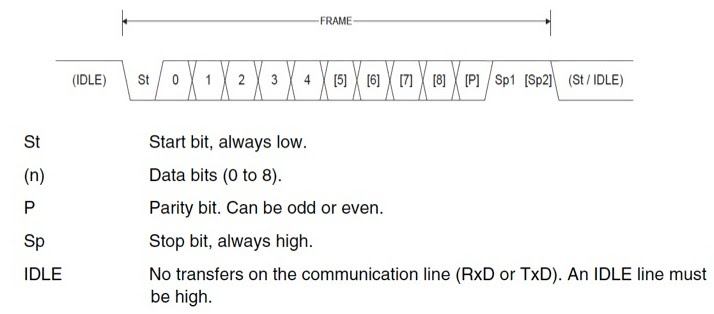
\includegraphics[scale=0.5]{fig/uart.jpg}
    \caption{Resumen protocolo UART.}
    \label{fig:mesh1}
\end{figure}

Para poder llevar a cabo una correcta depuración se ha utilizado un software llamado hercules, el cual permite poder establecer una comunicación entre el ordenador desde el cual se esté trabajando y el dispositivo con el cual se desee comunicar. De este modo, se pueden obtener información para poder conocer en que punto de cada función está en cada momento el código ejecutado y poder mostrar en pantalla la información necesaria para su correcta depuración.

\begin{figure}[h]
    \centering
    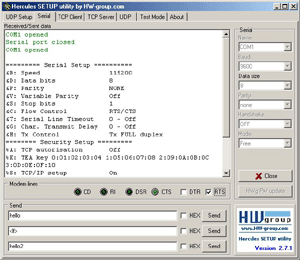
\includegraphics[scale=1.5]{fig/serial1.png}
    \caption{Comucicación serie en Hercules.}
    \label{fig:mesh1}
\end{figure}

El ordenador donde se esté ejecutando el software Hercules debe de poder interpretar la información a través de un USB, por tanto es necesario convertir esa información proveniente de un protocolo UART a un protocolo serie que pueda entender el ordenador.

En este caso se ha utilizado un adaptador capaz de convertir esta información para que pueda establecerse una comunicación en ambos canales y sentidos. El adaptador utilizado se puede encontrar en la siguiente figura.

\begin{figure}[h]
    \centering
    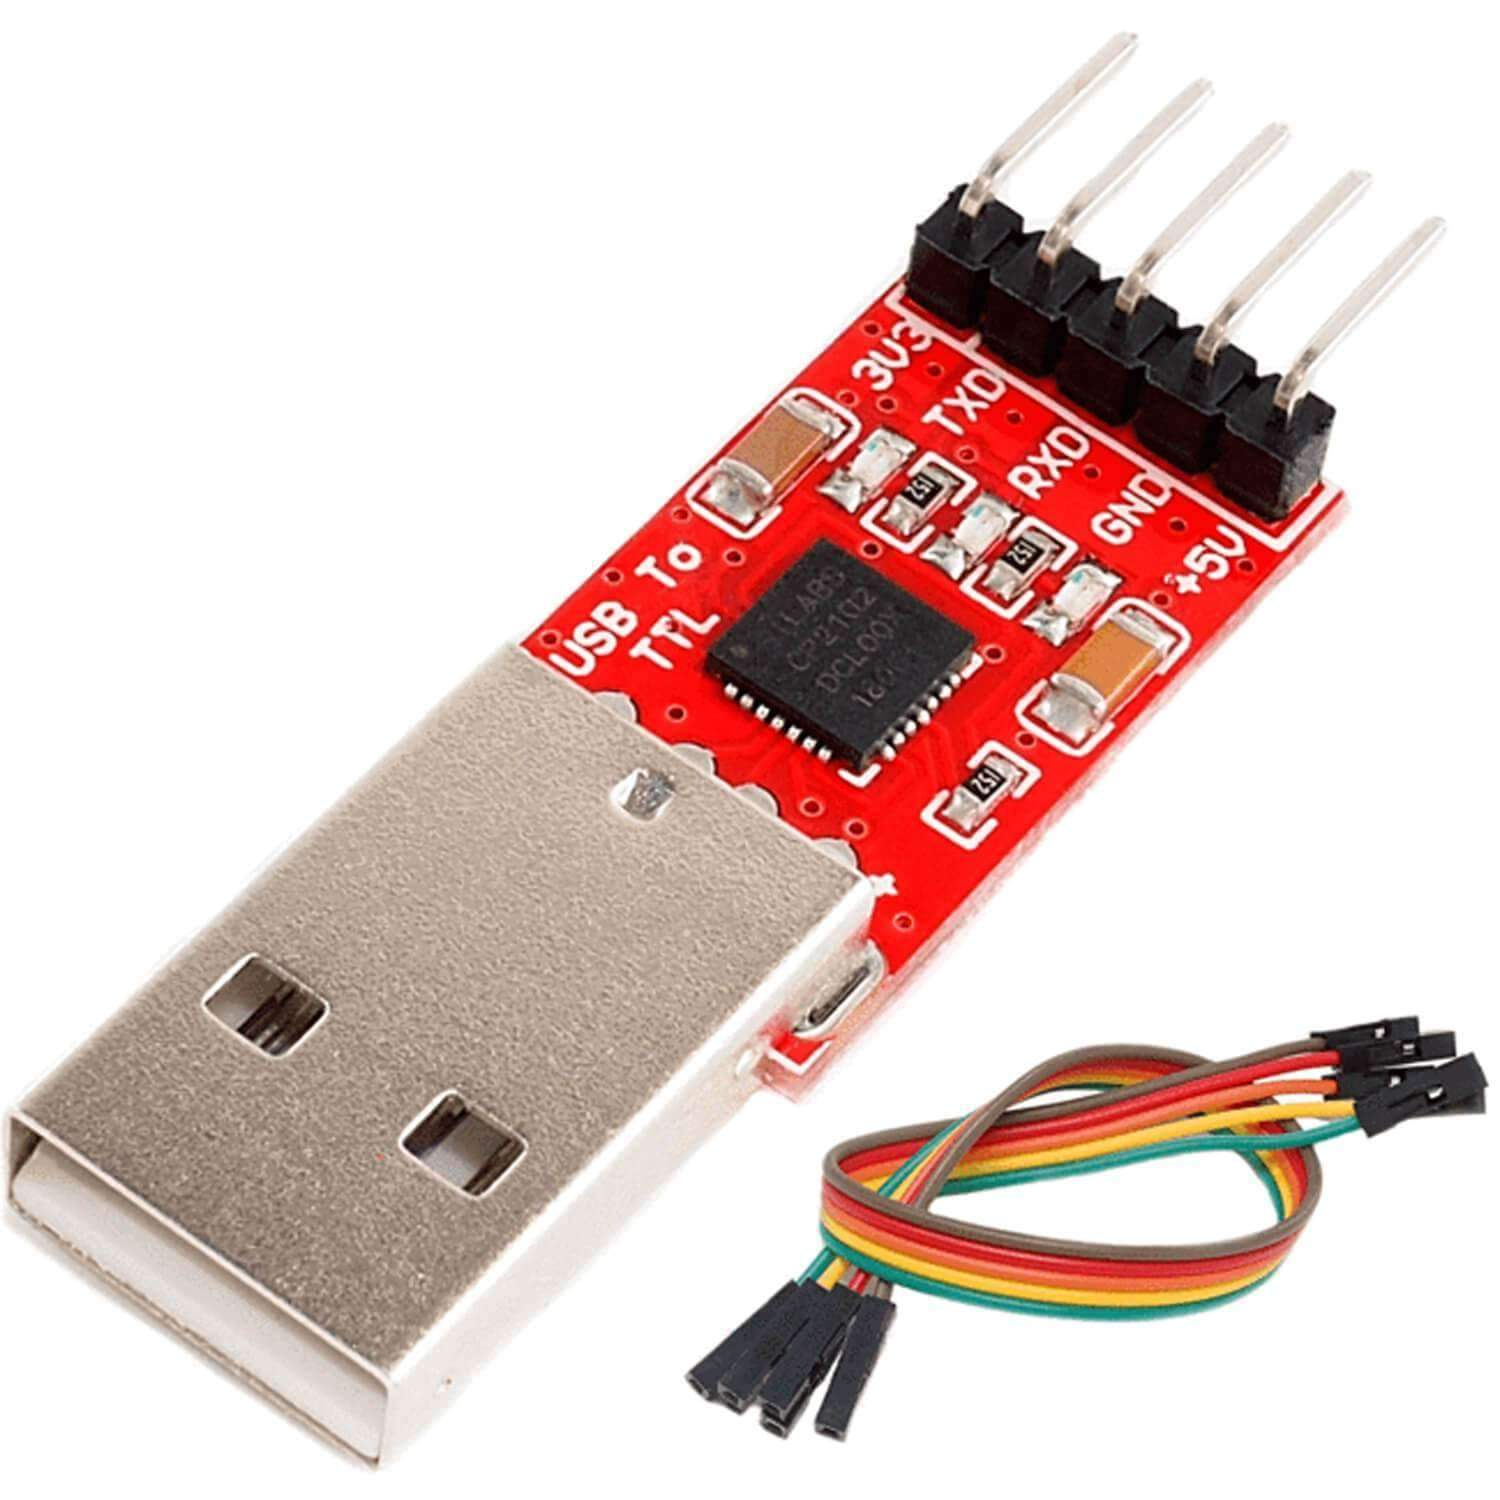
\includegraphics[scale=0.1]{fig/usb_ttl.jpg}
    \caption{Conversor USB-TTL.}
    \label{fig:mesh1}
\end{figure}

Otra herramienta que resulta muy útil a la hora de poder identificar problemas y poder depurar proyectos son los analizadores lógicos. Estos dispositivos permiten poder hacer un análisis a nivel de pines de cada uno de los canales o flujos que se quieran analizar en un proyecto. En ciertas circunstancias, cuando los dispositivos que s están programando no cuentan con herramientas propias de depuración con las que poder monitorizar "logs" o simplemente se quiere cerciorar que el flujo de comunicación funciona de forma correcta. Cualquier canal de comunicación o cualquier pista eléctrica que pueda conducir cualquier tipo de señal puede ser analizada con el analizador lógico, es aquí donde reside la versatilidad de este dispositivo. 

Hay distintos ámbitos en los que un analizador lógico puede ser útil en este proyecto, y en este caso se ha utilizado de diferentes maneras. EL dispositivo utilizado para el proyecto es un analizador lógico genérico que es fácil de encontrar en cualquier tienda de electrónica y con un precio bastante accesible a la mayor parte de los usuarios. El dispositivo se muestra en la figura siguiente.

\begin{figure}[h]
    \centering
    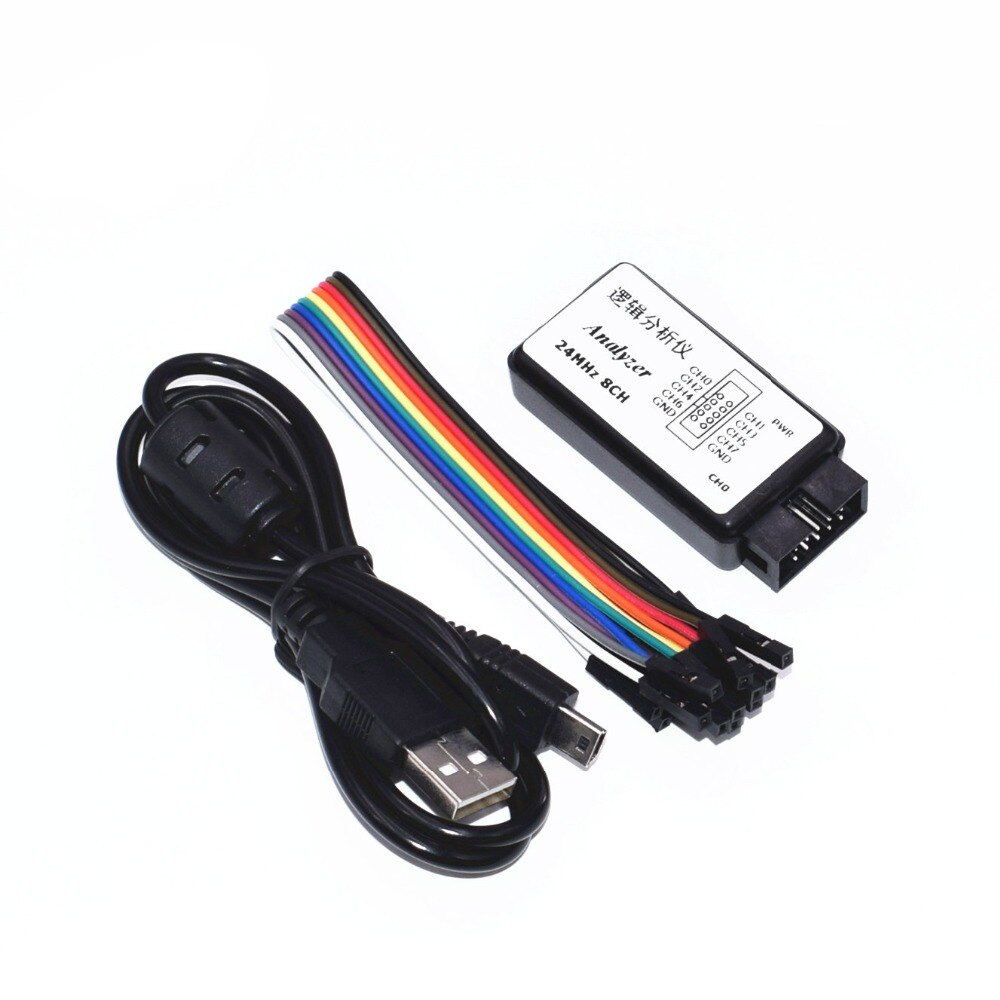
\includegraphics[scale=1]{fig/logic_analyzer.jpg}
    \caption{Analizador lógico utilizado en el proyecto.}
    \label{fig:mesh1}
\end{figure}

Para hacer uso del analizador lógico se necesita un software específico para interpretar la información adquirida por cada uno de los canales del analizador lógico. En este caso se ha utilizado un software libre y abierto llamado sigrok-pulseview, al cual se le deben de instalar los drivers compatibles con el dispositivo que se desea utilizar para poder completar la instalación y poder tener el dispositivo en pleno funcionamiento. Se puede encontrar un ejemplo de funcionamiento en la imagen siguiente.

\begin{figure}[h]
    \centering
    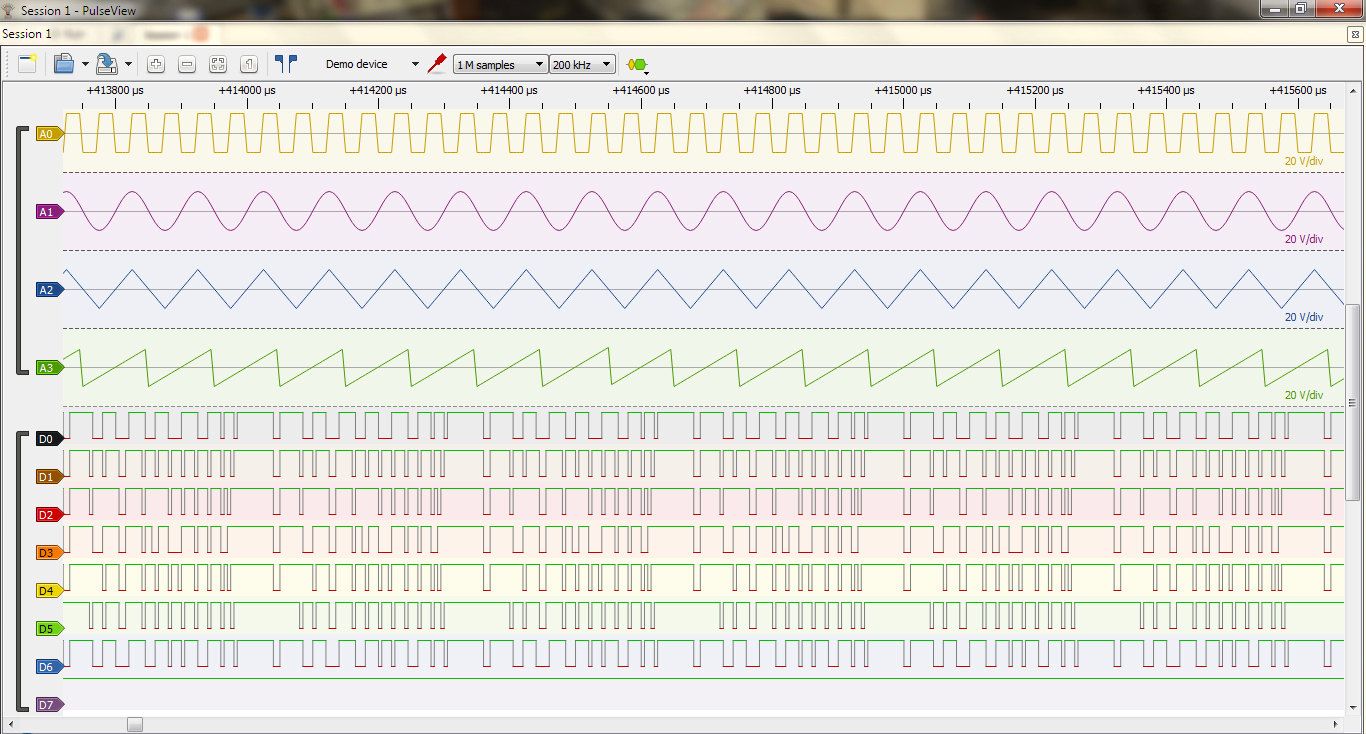
\includegraphics[scale=0.3]{fig/pulseview.jpg}
    \caption{Analizador lógico utilizado en el proyecto.}
    \label{fig:mesh1}
\end{figure}

\subsection{Docker Containers}

Con el propósito de poder replicar el funcionamiento del robot en todos los escenarios posibles de desarrollo, se ha tratado de utilizar un contenedor Docker.
Los contenedores Docker, son utilizados para encapsular y poder replicar y escalar un entorno de desarrollo determinado, donde todos y cada uno de los usuarios que utilicen dicho entorno, puedan tener las mismas herramientas disponibles para dicho desarrollo.

El modelo de robot escogido es el "rosbot description". Este modelo simula un robot de 2 ejes y cuatro ruedas implementado con una sensórica muy similar a la que se va a utilizar en el proyecto.
\subsection{Bash Scripting}

Con el objetivo de comprender como se realiza la detección de objetos, se han de dominar previamente diversos conceptos claves sobre los modelos de inteligencia artificial que se pueden encontrar actualmente en la red y disponen de la capacidad de poder embeberlos en un sistema que sea capaz de procesar esta información en el hardware que lleve el robot utilizado para el proyecto.

El modelo mas utilizado para la detección y segmentación de objetos relacionados con la robótica suelen ser las redes neuronales. Las redes neuronales favorecen el ajuste de una determinada 
     \chapter{Puesta en Marcha Laboratorio}\label{cap:implementacion}

\section {Herramientas}

\section{Conclusión}
En este capítulo concluimos que...
     \chapter{Conclusiones}\label{cap:implementacion}

\section{Conclusión general}
En este capítulo explicaremos...

\section {Propuesta de futuro}
     \chapter{Conclusiones}\label{cap:conclusiones}



    % Bibliografía
    \bibliographystyle{plainnat}
    \bibliography{bibliografia.bib}

% Fin del documento
\end{document}
